\section{Propiedades}

\subsection{El estado máxima entropía es separable}

Sea $\rho$ como en (\ref{eq:rhoz}), entonces por (\ref{eq:MaxEnt}) el estado de máxima entropía es:
\begin{equation}\label{eq:MaxEntUgly}
\varrho_{max}=\frac{\text{exp}(-\lambda_{3}\hat{G}_{3})}{\Tr[\text{exp}(-\lambda_{3}\hat{G}_{3})]}
\end{equation}
donde $\hat{G}_{3}$ se define según (\ref{eq:Gop}). Como los dos términos que componen al operador comuntan entre sí, la exponencial puede separarse:
\begin{align*}
\varrho_{max}&=\frac{1}{Z}e^{-\lambda_{3}p\sigma_{z}\otimes\Id}e^{-\lambda_{3}(1-p)\Id\otimes\sigma_{z}}\\
&=\frac{1}{Z}(e^{-\lambda_{3}p\sigma_{z}}\otimes\Id)( \Id\otimes e^{-\lambda_{3}(1-p)\sigma_{z}})\\
&=\frac{1}{Z}(e^{-\lambda_{3}p\sigma_{z}}\otimes e^{-\lambda_{3}(1-p)\sigma_{z}})\\
\end{align*}
Si se separa a la función de partición como un producto de trazas $Z=Z_{1}Z_{2}$, al estado de máxima entropía se le puede escribir como:
\begin{equation}\label{eq:MaxEntZ}
\varrho_{max}=\frac{e^{-\lambda_{3}p\sigma_{z}}}{Z_{1}} \otimes \frac{e^{-\lambda_{3}(1-p)\sigma_{z}}}{Z_{2}}
\end{equation}

\subsection{El estado de máxima entropía bajo la aplicación de grano grueso}

El problema de la ecuación (\ref{eq:MaxEntZ}) es que el estado de máxima entropía está en términos del multiplicador de Lagrange que se usó para maximizar la entropía, en lugar de estar en términos de la cantidad medible $r_{z}$. Si por alguna razón tuviéramos que resignarnos a trabajar con el estado en términos de $\lambda$, será necesario conocer la expresión del estado efectivo. Para hallarla, basta con pasar (\ref{eq:MaxEntZ}) por la aplicación de grano grueso. El estado efectivo es 
\begin{equation}\label{eq:CG(MaxEntZ)1}
    \rho=\frac{1}{Z}\CG{\varrho_{max}}=p\frac{e^{-\lambda_{3}p\sigma_{z}}}{Z_{1}}+(1-p)\frac{e^{-\lambda_{3}(1-p)\sigma_{z}}}{Z_{2}},
\end{equation}
Las exponenciales de la ecuación (\ref{eq:CG(MaxEntZ)1}) pueden verse como $e^{a\hat{n}\cdot \vec{\sigma}}$. Si se desarollan las series se halla
\begin{equation}\label{eq:PauliVectorExp}
    e^{a\hat{n}\cdot \vec{\sigma}}=\Id \cosh{a}+(\hat{n}\cdot \vec{\sigma})\sinh{a}
\end{equation}
así que, sustituyendo la ecuación (\ref{eq:PauliVectorExp}) en (\ref{eq:CG(MaxEntZ)1}) se encuentra la expresión del estado efectivo en términos de la base de Pauli
\begin{align*}
    \rho&=p\frac{\Id \cosh{\lambda_{3}p}-\sigma_{z}\sinh{\lambda_{3}p}}{Z_{1}}+(1-p)\frac{\Id \cosh{\lambda_{3}(1-p)}-\sigma_{z}\sinh{\lambda_{3}(1-p)}}{Z_{2}}\\
    &=p\frac{1}{2}(\Id \frac{2\cosh{\lambda_{3}p}}{Z_{1}}+\sigma_{z}\frac{2\sinh{\lambda_{3}p}}{Z_{1}})+(1-p)\frac{1}{2}(\Id \frac{2\cosh{\lambda_{3}(1-p)}}{Z_{2}}+\sigma_{z}\frac{2\sinh{\lambda_{3}(1-p)}}{Z_{2}})
\end{align*}
para que esto sea de la forma $\rho=\sum_{i}p_{i}\rho_{i}$ es necesario que $Z_{1}=2\cosh{\lambda p}$ y $Z_{2}=2\cosh{\lambda (1-p)}$ (cosa que se puede comprobar). El estado efectivo en términos de $\lambda_{3}$ es
\begin{equation}\label{eq:CG(MaxEntZ)2}
    \rho=p\frac{1}{2}(\Id+\sigma_{z}\tanh{\lambda p})+(1-p)\frac{1}{2}(\Id+\sigma_{z}\tanh{\lambda (1-p)})
\end{equation}


\subsection{El estado de máxima entropía en términos de $r_{z}$}
La ecuación (\ref{eq:CG(MaxEntZ)2}) permite expresar la coordenada $r_{z}$ en términos del multiplicador de Lagrange complejo es
\begin{equation}\label{eq:RzTanh}
    r_{z}=p\tanh{\lambda p}+(1-p)\tanh{\lambda (1-p)}.
\end{equation}
Esta expresión la obtuve después de ahaber desarollado los párrafos de discusión que siguen. 
La forma matricial de este estado es:
\begin{equation*}
\left(
\begin{array}{cccc}
 \frac{1}{4} e^{-\lambda_{3}} \text{sech}(\lambda_{3} p)
   \text{sech}(\lambda_{3}-\lambda_{3} p) & 0 & 0 & 0 \\
 0 & \frac{e^{2 \lambda_{3}}}{\left(e^{2 \lambda_{3}
   p}+1\right) \left(e^{2 \lambda_{3}}+e^{2 \lambda_{3}
   p}\right)} & 0 & 0 \\
 0 & 0 & \frac{1}{\left(e^{2 \lambda_{3}}+1\right) e^{-2
   \lambda_{3} p}+e^{2 \lambda_{3}-4 \lambda_{3}
   p}+1} & 0 \\
 0 & 0 & 0 & \frac{1}{4} e^{\lambda_{3}}
   \text{sech}(\lambda_{3} p) \text{sech}(\lambda_{3}-\lambda_{3} p) \\
\end{array}
\right)
\end{equation*}
Hallar el valor de $\lambda_{
3}$ en términos del valor $r_{z}$ implica resolver la ecuación:
\begin{equation}\label{eq:RZ}
rz=-\frac{1}{2}\frac{\sinh(\lambda_{3})+(1-2p)\sinh((1-2p)\lambda_{3})}{\cosh(p\lambda_{3})\cosh((1-p)\lambda_{3})}
\end{equation}
No se ve ninguna forma sencilla de despejar al multiplicador de Lagrange \notaAd{la ecuación (\ref{eq:RzTanh}) y la ecuación (\ref{eq:RZ}) son completamente equivalentes, como debería de ser. La segunda siendo más fea que la primera. }. En realidad, esto solo se puede si la función $r_{z}(\lambda_{3})$ tiene inversa, y esto puede depender del parámetro $p$. Graficar la superficie (Figura \ref{fig:rzsurf}) puede aclarar algo el panorama.
\begin{figure}[h!]
\centering
\begin{subfigure}{0.475\textwidth}
  \centering
  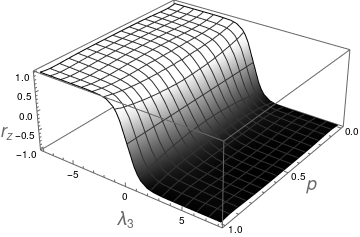
\includegraphics[width=0.6\linewidth]{maxent/figures/LagrangeMult_lambda-8to8.png}
  \caption{$-8<\lambda_{3}<8$}
\end{subfigure}%
\begin{subfigure}{0.475\textwidth}
  \centering
  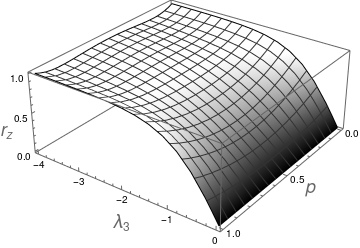
\includegraphics[width=0.6\linewidth]{maxent/figures/LagrangeMult_lambda-4to0.png}
  \caption{$-4<\lambda_{3}<0$}
\end{subfigure}
\caption{Superficie de $r_{z}$ según (\ref{eq:RZ}) para dos intervalos de $\lambda_{3}$. A valores $\lambda_{3}<0$ corresponden valores $r_{z}>0$ y viceversa.}
\label{fig:rzsurf}
\end{figure}

Después de una breve inspección se concluyen las siguientes cosas:
\begin{itemize}
\item la superficie es simétrica respecto al plano $p=0.5$
\item la superficie es antisimétrica  respecto al plano $\lambda_{3}=0$ i.e. $r_{z
}(\lambda_{3},p)=-r_{z
}(-´\lambda_{3},p)$
\item $\text{sgn}(\lambda_{3})=-\text{sgn}(r_{z})$
\end{itemize}

La simetría respecto al plano $p=0.5$ suguiere un cambio de variable $q=\abs{p-0.5}$. La ecuación (\ref{eq:RZ}) se reescribe como:
\begin{equation}\label{eq:RZq}
r_{z}=-\frac{1}{2}\frac{\sinh(\lambda_{3})+2q\sinh(2q\lambda_{3})}{\cosh((q+\frac{1}{2})\lambda_{3})\cosh((q-\frac{1}{2})\lambda_{3})}
\end{equation}
Y nos limitamos al dominio $\lambda_{3}\leq0$ y $0\leq q\leq\frac{1}{2}$. Podemos graficar la función (\ref{eq:RZq}) para diferentes valores de $q$ (Figura \ref{fig:rzinv}).
\begin{figure}[h!]
\centering
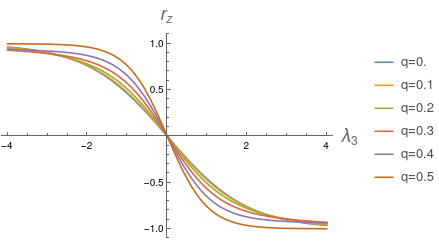
\includegraphics[width=0.6\linewidth]{maxent/figures/rz_has_inverse_lambda-4to4.png}
\caption{$r_{z}$ como función de $\lambda_{3}$ para diferentes valores de $q$. La apariencia uno a uno sugiere la existencia de una inversa.}
\label{fig:rzinv}
\end{figure}

\subsubsection{Dos soluciones particulares}

Considerando el caso $q=\frac{1}{2}$, la ecuación (\ref{eq:RZq}) se reduce a 
\begin{equation}
r_z=-\frac{1}{2}\frac{2\sinh(\lambda_{3})}{\cosh(\lambda_{3})}
\end{equation}
de manera que $\lambda_{3}=-\text{arctanh}(rz)$.

Si $q=0$, la ecuación (\ref{eq:RZq}) se reduce a
\begin{equation}
r_z=-\frac{\sinh(\lambda_{3})}{\cosh(\lambda_{3}+1)}
\end{equation}
Mathematica sugiere la solución:
\begin{equation}\label{eq:lambda0.5}
\lambda_{3}=\log\qty(\frac{1-r_{z}}{1+r_{z}}).
\end{equation}